\documentclass{ximera}

\input{../preamble.tex}

\outcome{Compute volumes using the shell method.}
\outcome{Know when to use the shell method.}
\outcome{Set up integrals for the computing volume using the shell method.}

\title[Dig-In:]{Accumulated shells}

\begin{document}
\begin{abstract}
Some volumes of revolution are more easily computed with cylindrical shells. 
\end{abstract}
\maketitle


\section{More than one method}

Rylee, In this section, we will show you a new method for computing volumes
of solids of revolution.  Consider the following region bounded by
$f(x)=x+1$ and $g(x)=(x-1)^2$:
\begin{image}
\begin{tikzpicture}
  \begin{axis}[
      xmin=0, xmax=3,domain=0:3,
      clip=false,
      axis lines =center, xlabel=$x$, ylabel=$y$,
      every axis y label/.style={at=(current axis.above origin),anchor=south},
      every axis x label/.style={at=(current axis.right of origin),anchor=west},
      axis on top,
    ]
    \addplot [draw=none,fill=fillp] {x+1}\closedcycle;
    \addplot [draw=none,fill=white] {(x-1)^2}\closedcycle;
    \addplot [penColor,very thick] {x+1};
    \addplot [penColor2,very thick] {(x-1)^2};

    \node at (axis cs:2,3.3) [penColor] {$f$};
    \node at (axis cs:2.5,1.7) [penColor2] {$g$};
  \end{axis}
\end{tikzpicture}
\end{image}
If this region is rotated around the $y$-axis, it is possible, but
inconvenient, to compute the volume of the resulting solid by the
methods we have used so far. The issue is that there are two
"kinds'' of cylindrical cross-sections: 
\begin{image}
\begin{tikzpicture}
  \begin{axis}[
      xmin=-3, xmax=3,
      clip=false,
      width=4in,
      height=2in,
      axis lines =center, xlabel=$x$, ylabel=$y$,
      every axis y label/.style={at=(current axis.above origin),anchor=south},
      every axis x label/.style={at=(current axis.right of origin),anchor=west},
      axis on top,
    ]
    \addplot [penColor,very thick,domain=0:1] {x+1};
    \addplot [penColor,very thick,domain=-1:0] {-x+1};
    \addplot [penColor2,very thick,domain=-3:-.25] {(-x-1)^2};
    \addplot [penColor2,very thick,domain=.25:3] {(x-1)^2};
    
    \draw[penColor,very thick,fill=fillp] (axis cs:0,1.9) ellipse (240 and 20);
    \draw[penColor,very thick,fill=fillp] (axis cs:0,2) ellipse (240 and 20);
    \draw[penColor,very thick,fill=white] (axis cs:0,2) ellipse (100 and 10);

    \draw[penColor,very thick,fill=fillp] (axis cs:0,.46) ellipse (175 and 20);
    \draw[penColor,very thick,fill=fillp] (axis cs:0,.56) ellipse (175 and 20);
    \draw[penColor,very thick,fill=white] (axis cs:0,.56) ellipse (25 and 5);

    
    \addplot [penColor,very thick,domain=1:3] {x+1};
    \addplot [penColor2,very thick,domain=0:.25] {(x-1)^2};
    \addplot [penColor,very thick,domain=-3:-1] {-x+1};
    \addplot [penColor2,very thick,domain=-.25:0] {(-x-1)^2};

    \node at (axis cs:2,3.3) [penColor] {$f$};
    \node at (axis cs:2.5,1.7) [penColor2] {$g$};
    \node at (axis cs:-2.7,2) {$\d y$};

    \draw[decoration={brace,raise=.1cm},decorate,thin] (axis cs:-2.4,1.8)--(axis cs:-2.4,2.1);
    
    \addplot [very thick, penColor4] plot coordinates {(.25,.56) (1.75,.56)};
    \addplot [very thick, penColor4] plot coordinates {(1,2) (2.41,2)};
    
    \end{axis}
\end{tikzpicture}
%% \caption{A plot of $f(x) = x+1$ and $g(x) = (x-1)^2$ with the two
%%   types of ``washers'' indicated.}
%% \label{figure:washerHARD}
\end{image}
As we see above, some of the cylindrical cross sections are defined
by the line that goes from $g$ to $f$, and others are defined by the
line that touches $g$ at both ends.  To compute the volume using
accumulated cross-sections, we need to break the problem into two
integrals:
\begin{itemize}
  \item an integral that computes the volume of the region bounded by
    $g$ and the line $y=1$, rotated about the $y$-axis, and
  \item an integral that computes the volume of the region bounded by
    $f$, $g$ and the line $y=1$, rotated about the $y$-axis.
\end{itemize}
Since we are rotating around the $y$-axis, we should look at $f^{-1}$
and $g^{-1}$.
\begin{explanation}
  Write with me:
  \[
  f^{-1}(y) = \answer[given]{y-1}
  \]
  On the other hand $g$ is \textbf{not} \index{one-to-one}one-to-one, so
  we cannot invert it on the entire domain. Nevertheless, if we restrict
  the domain of $g$ we may write two separate functions
  \[
  g^{-1}_1(y) = \answer[given]{1-\sqrt{y}}\qquad\text{when $0<x<1$}
  \]
  and
  \[
  g^{-1}_2(y) = \answer[given]{1+\sqrt{y}}\qquad\text{when $1<x<3$}.
  \]
\end{explanation}
With this in mind, we can compute our volume with:
\begin{align*}
  \int_0^1 &\pi(g^{-1}_2(y))^2-\pi(g_1^{-1}(y))^2\d y\\
  &+ \int_1^4\pi(g^{-1}_2(y))^2-\pi(f^{-1}(y))^2\d y
\end{align*}
\begin{explanation}
Substituting in, we find
  \begin{align*}
    =\int_0^1 &\pi(1+\sqrt{y})^2-\answer[given]{\pi(1-\sqrt{y})^2}\d y\\
    &+ \int_1^4  \pi(1+\sqrt{y})^2-\answer[given]{\pi(y-1)^2}\d y
  \end{align*}
  and so
  \begin{align*}
  &=\frac{8\pi}{3} + \frac{65\pi}{6}\\
  &=\answer[given]{\frac{27\pi}{2}}.
  \end{align*}
\end{explanation}
While we have successfully solved this problem, it wasn't easy. Let's
see another, perhaps easier method to solve this problem.  If instead
we consider a vertical rectangle of height $f(x)-g(x)$ (just like we
did when we computed areas of regions between curves!)  and width $\d
x$, and we additionally rotate this rectangle around the $y$-axis, we
get a thin ``shell'' or hollow-tube:
\begin{image}
\begin{tikzpicture}
  \begin{axis}[
      xmin=-3, xmax=3,domain=0:3,
      clip=false,
      width=4in,
      height=2in,
      axis lines =center, xlabel=$x$, ylabel=$y$,
      every axis y label/.style={at=(current axis.above origin),anchor=south},
      every axis x label/.style={at=(current axis.right of origin),anchor=west},
      axis on top,
    ] 
   

    \addplot [draw=none,fill=fillp!50!white] plot coordinates {(1.5,2.5) (1.5,.25) (-1.5,.25) (-1.5,2.5)};
    
    \draw[penColor,very thick,fill=fillp] (axis cs:0,2.5) ellipse (150 and 20);
    \draw[penColor,very thick,fill=white] (axis cs:0,2.5) ellipse (120 and 10);
    
   \draw[penColor, very thick,dashed, fill=fillp!50!white] (axis cs:0,0.25) ellipse (150 and 20);
   \draw[penColor, very thick, dashed,fill=white] (axis cs:0,0.25) ellipse (120 and 10);
   
     \addplot [penColor,very thick,domain=-3:0] {-x+1};
   \addplot [penColor2,very thick,domain=-3:0] {(-x-1)^2};
   
   \addplot [penColor,very thick] {x+1};
   \addplot [penColor2,very thick] {(x-1)^2};

    \node at (axis cs:2,3.3) [penColor] {$f$};
    \node at (axis cs:2.5,1.7) [penColor2] {$g$};

    
    \node at (axis cs:1.35,3) {$\d x$};
    \draw[decoration={brace,raise=.1cm},decorate,thin] (axis cs:1.2,2.6)--(axis cs:1.5,2.6);
    
    \addplot [very thick, penColor4] plot coordinates {(1.5,2.5) (1.5,.25)};
    \addplot [very thick, penColor4] plot coordinates {(-1.5,2.5) (-1.5,.25)};
    \addplot [very thick, penColor4, dashed] plot coordinates {(1.2,2.5) (1.2,.25)};
    \addplot [very thick, penColor4, dashed] plot coordinates {(-1.2,2.5) (-1.2,.25)};
    \draw[very thick, penColor]   (axis cs: -1.5,.25) arc(180:360:150 and 20);
  \end{axis}
\end{tikzpicture}
%% \caption{A plot of $f(x) = x+1$ and $g(x) = (x-1)^2$ with the
%%   ``shell'' indicated.}
%% \label{figure:shellIndicated}
\end{image}
Here the infinitesimal change in volume is:
\begin{image}
  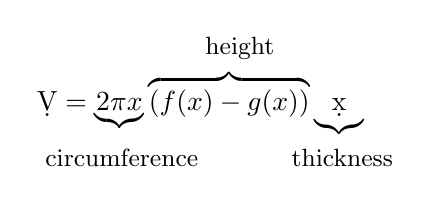
\begin{tikzpicture}
    \node at (0,0) {
      $\d V = \underbrace{2\pi x} \overbrace{(f(x)- g(x))}\underbrace{\d x}$
    };
    \node at (-1,-.7) {\small{circumference}};
    \node at (.5,.7) {\small{height}};
    \node at (1.8,-.7) {\small{thickness}};
  \end{tikzpicture}
\end{image}
Integrating $\d V$ will give us our desired volume.

%% What is the volume of such a shell?  Consider the shell at $x$.
%% Imagine that we cut the shell vertically in one place and ``unroll''
%% it into a thin, flat sheet. This sheet will be $f(x)-g(x)$ tall, and
%% $2\pi x$ wide since this is the circumference of the shell before it
%% was unrolled.  We may now write the integral


%% \begin{image}
%%   \begin{tikzpicture}
%%     \begin{axis}[
%%           xmin =0,xmax=4,ymax=5,ymin=-5,
%%           axis lines=none, xlabel=$x$, ylabel=$y$,
%%           every axis y label/.style={at=(current axis.above origin),anchor=south},
%%           every axis x label/.style={at=(current axis.right of origin),anchor=west},
%%           axis on top,
%%           width=5in,
%%           xtick={0,6}, xticklabels={$0$, $20$},
%%           ytick={0,3},yticklabels={$0$,$20$},
%%             clip=false,
%%       ]

            
%%       %\addplot [draw=penColor, thick] plot coordinates {(-3,-3) (0,0)};
%%       %\addplot [draw=penColor, thick] plot coordinates {(6,0) (0,0)};
%%       %\addplot [draw=penColor, thick] plot coordinates {(1.5,3) (3,-3)};
%%       %\addplot [draw=penColor, thick] plot coordinates {(1.5,3) (0,0)};

%%       %% slab
%%       \addplot [draw=penColor, fill=fillp,very thick] plot coordinates {(3,2) (1,2) (0,1) (2, 1) (3,2)};
%%       \addplot [draw=penColor, fill=fillp,very thick] plot coordinates {(0,.8) (0,1) (2,1) (2, .8) (0,.8)};
%%       \addplot [draw=penColor, fill=fillp,very thick] plot coordinates {(2,1) (2, .8) (3,1.8) (3,2) (2,1)};

%%       %\addplot [draw=penColor, fill=fillp,very thick] plot coordinates {(3,1.8) (1,1.8) (0,.8) (2, .8) (3,1.8)};
%%       %\addplot [draw=penColor, fill=fillp,very thick] plot coordinates {(3,2) (1,2) (0,1) (2, 1) (3,2)};



%%       \draw[decoration={brace,mirror,raise=.1cm},decorate,thin] (axis cs:0,.8)--(axis cs:2,.8);
%%       \draw[decoration={brace,mirror,raise=.1cm},decorate,thin] (axis cs:2,.8)--(axis cs:3,1.8);
%%       \draw[decoration={brace,raise=.1cm},decorate,thin] (axis cs:3,2.05)--(axis cs:3,1.75);
      
%%      % \addplot [->] plot coordinates {(0,0) (-4,-4)};
%%       %\node[anchor=north east] at (axis cs:-4,-4) {$z$};

%%       \node at (axis cs:3.15,1.9) {$\d x$};
%%       \node at (axis cs:2.8,0.8) {$f(x)-g(x)$};
%%       \node at (axis cs:1,.4) {$2x\pi$};       
%%     \end{axis}
%%   \end{tikzpicture}
%% \end{image}

\section{Shells around the axes}\index{shells}


Let's start by actually doing our motivating example above.


\begin{example}
  Consider the region below bounded by $f(x)=x+1$ and $g(x)=(x-1)^2$:
\begin{image}
\begin{tikzpicture}
  \begin{axis}[
      xmin=0, xmax=3,domain=0:3,
      clip=false,
      axis lines =center, xlabel=$x$, ylabel=$y$,
      every axis y label/.style={at=(current axis.above origin),anchor=south},
      every axis x label/.style={at=(current axis.right of origin),anchor=west},
      axis on top,
    ]
    \addplot [draw=none,fill=fillp] {x+1}\closedcycle;
    \addplot [draw=none,fill=white] {(x-1)^2}\closedcycle;
    \addplot [penColor,very thick] {x+1};
    \addplot [penColor2,very thick] {(x-1)^2};

    \node at (axis cs:2,3.3) [penColor] {$f$};
    \node at (axis cs:2.5,1.7) [penColor2] {$g$};
  \end{axis}
\end{tikzpicture}
\end{image}
  Find the volume of the solid of revolution formed by rotating this
  region around the $y$-axis.
  \begin{explanation}
    We'll solve this problem using accumulated shells. If we draw our shell, we see
    \begin{image}
\begin{tikzpicture}
  \begin{axis}[
      xmin=-3, xmax=3,domain=0:3,
      clip=false,
      width=4in,
      height=2in,
      axis lines =center, xlabel=$x$, ylabel=$y$,
      every axis y label/.style={at=(current axis.above origin),anchor=south},
      every axis x label/.style={at=(current axis.right of origin),anchor=west},
      axis on top,
    ] 
   

    \addplot [draw=none,fill=fillp!50!white] plot coordinates {(1.5,2.5) (1.5,.25) (-1.5,.25) (-1.5,2.5)};
    
    \draw[penColor,very thick,fill=fillp] (axis cs:0,2.5) ellipse (150 and 20);
    \draw[penColor,very thick,fill=white] (axis cs:0,2.5) ellipse (120 and 10);


   \draw[penColor, very thick, dashed, fill=fillp!50!white] (axis cs:0,0.25) ellipse (150 and 20);
   \draw[penColor, very thick, dashed,fill=white] (axis cs:0,0.25) ellipse (120 and 10);


     \addplot [penColor,very thick,domain=-3:0] {-x+1};
   \addplot [penColor2,very thick,domain=-3:0] {(-x-1)^2};
   
   \addplot [penColor,very thick] {x+1};
   \addplot [penColor2,very thick] {(x-1)^2};

    \node at (axis cs:2,3.3) [penColor] {$f$};
    \node at (axis cs:2.5,1.7) [penColor2] {$g$};

    
    \node at (axis cs:1.35,3) {$\d x$};
    \draw[decoration={brace,raise=.1cm},decorate,thin] (axis cs:1.2,2.6)--(axis cs:1.5,2.6);
    
    \addplot [very thick, penColor4] plot coordinates {(1.5,2.5) (1.5,.25)};
    \addplot [very thick, penColor4] plot coordinates {(-1.5,2.5) (-1.5,.25)};
    \addplot [very thick, penColor4, dashed] plot coordinates {(1.2,2.5) (1.2,.25)};
    \addplot [very thick, penColor4, dashed] plot coordinates {(-1.2,2.5) (-1.2,.25)};
    \draw[very thick, penColor]   (axis cs: -1.5,.25) arc(180:360:150 and 20);
  \end{axis}
\end{tikzpicture}
%% \caption{A plot of $f(x) = x+1$ and $g(x) = (x-1)^2$ with the
%%   ``shell'' indicated.}
%% \label{figure:shellIndicated}
    \end{image}
    Since the volume of each shell is
    \[
    \d V = 2\pi x (f(x) -g(x) ) \d x
    \]
    we may write 
    \begin{align*}
      \int_{\answer[given]{0}}^{\answer[given]{3}} 2\pi x(f(x)-g(x))\d x &= \int_{\answer[given]{0}}^{\answer[given]{3}} 2\pi x(\answer[given]{x+1}-(x-1)^2)\d x\\
      &= \eval{\answer[given]{2\pi x^3 -\frac{\pi x^4}{2}}}_{\answer[given]{0}}^{\answer[given]{3}}\\
      &=\answer[given]{\frac{27\pi}{2}}.
    \end{align*}
  \end{explanation}
\end{example}


Comparing our work above to our earlier work, we see that using shells
not only solves the problem with just one integral, we see that the
integral itself is somewhat easier than those in the previous
calculation! Things are not always so neat, but it is often the case
that one of the two methods will be simpler than the other, so it is
worth considering both methods.


\begin{example} 
Suppose the area bounded by $y=\sqrt{x}$, the line $y = 2x-1$, and the
$x$-axis is rotated around the $x$-axis,
\begin{image}
\begin{tikzpicture}
  \begin{axis}[
      xmin=0, xmax=1.2,ymax = 1.7, ymin = -.5,domain=0:1.2,
      clip=true,
      axis lines =center, xlabel=$x$, ylabel=$y$,
      every axis y label/.style={at=(current axis.above origin),anchor=south},
      every axis x label/.style={at=(current axis.right of origin),anchor=west},
      axis on top,
    ] 
  \addplot [draw=none,fill=fillp, domain=0:1] {sqrt(x)}\closedcycle;
    \addplot [penColor,very thick, samples = 100,smooth] {sqrt(x)};
    \addplot [penColor2,very thick,domain=0.5:1.5] {2*x-1};
     \addplot [draw=none,fill=white,very thick,domain=0.5:1] {2*x-1.02}\closedcycle;
  \end{axis}
\end{tikzpicture}
\end{image}
find the volume of this solid.
\begin{explanation}
While we could use accumulated cross-sections to compute this volume,
it would require \textit{two} integrals, (the industrious young
mathematician is encouraged to attempt to solve this problem using
accumulated cross-sections). However, here we will use the method of
shells. Let's see a picture:
\begin{image}
\begin{tikzpicture}
  \begin{axis}[
      xmin=0, xmax=1.2,ymax = 1.7, ymin = -1.7,
      clip=true,
      axis lines =center, xlabel=$x$, ylabel=$y$,
      every axis y label/.style={at=(current axis.above origin),anchor=south},
      every axis x label/.style={at=(current axis.right of origin),anchor=west},
      axis on top,
    ] 

    \addplot [draw=none, fill=fill1!50!white] plot coordinates {(.8,.6) (.36,.6) (.36,-.6) (.8,-.6)};
    
    \draw[penColor,dashed,very thick,fill=fillp!50!white] (axis cs:.36,0) ellipse (7 and 60);
    \draw[penColor,dashed,very thick,fill=white] (axis cs:.36,0) ellipse (5 and 50);
    
    \addplot [very thick, penColor4] plot coordinates {(.8,.6) (.36,.6)};
    \addplot [very thick, penColor4] plot coordinates {(.8,-.6) (.36,-.6)};
    \addplot [very thick, penColor4, dashed] plot coordinates {(.8,.5) (.36,.5)};
    \addplot [very thick, penColor4, dashed] plot coordinates {(.8,-.5) (.36,-.5)};

    \addplot [penColor,very thick, samples = 100,smooth,domain=0:1.2] {sqrt(x)};
    \addplot [penColor2,very thick,domain=0.5:1.5] {2*x-1};
    \addplot [penColor,very thick, samples = 100,smooth,domain=0:1.2] {-sqrt(x)};
    \addplot [penColor2,very thick,domain=0.5:1.5,domain=.5:1.2] {-2*x+1};

    \draw[penColor,very thick,fill=fillp] (axis cs:.8,0) ellipse (7 and 60);
    \draw[penColor,very thick,fill=white] (axis cs:.8,0) ellipse (5 and 50);

    \draw[decoration={brace,raise=.1cm},decorate,thin] (axis cs:.85,.65)--(axis cs:.85,.45);
    \node at (axis cs:.92,.55) {$\d y$};
    \draw[very thick, penColor]   (axis cs: .36,.6) arc(90:270:7 and 60);
  \end{axis}
\end{tikzpicture}
\end{image}
In this case, the volume of each shell is
\begin{image}
  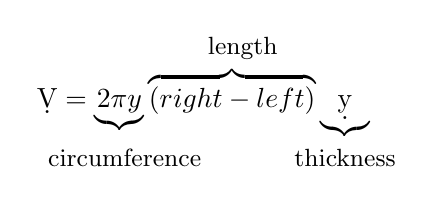
\begin{tikzpicture}
    \node at (0,0) {
      $\d V = \underbrace{2\pi y} \overbrace{(\text{right}-\text{left})}\underbrace{\d y}$
    };
    \node at (-1,-.7) {\small{circumference}};
    \node at (.5,.7) {\small{length}};
    \node at (1.8,-.7) {\small{thickness}};
  \end{tikzpicture}
\end{image}
Since we are integrating with respect to $y$, we have
\[
y=\sqrt{x} \qquad\Rightarrow\qquad x = \answer[given]{y^2}
\]
and
\[
y = 2x-1  \qquad\Rightarrow\qquad x= \answer[given]{\frac{y+1}{2}}.
\]
Hence the volume of our shell is
\[
\d V = 2\pi y \left(\answer[given]{\frac{y+1}{2} -y^2}\right) \d y
\]
Thus the the total volume of our solid of revolution is given by
\begin{align*}
  \text{Volume} &= \int_{\answer[given]{0}}^{\answer[given]{1}} \answer[given]{2\pi y (\frac{y+1}{2} - y^2)} \d y\\
  &= 2\pi\int_{\answer[given]{0}}^{\answer[given]{1}} \frac{y^2}{2}+\frac{y}{2} - y^3 \d y\\
  &= 2\pi\eval{\answer[given]{\frac{y^3}{6}+\frac{y^2}{4} - \frac{y^4}{4}}}_{\answer[given]{0}}^{\answer[given]{1}}\\
  &= \answer[given]{\frac{\pi}{3}}.
\end{align*}
\end{explanation}
\end{example}









\section{Shells around other lines}


What if we had wanted to rotate the region from the last example about
the line $y = -1$ instead of the $x$-axis? In this case, we draw a
picture and work much the same way as before. Let's see an example. 

\begin{example}
Suppose the area bounded by $y=\sqrt{x}$, the line $y = 2x-1$, and the
$x$-axis is rotated around the line $y= -1$,
\begin{image}
\begin{tikzpicture}
  \begin{axis}[
      xmin=0, xmax=1.2,ymax = 1.7, ymin = -.5,domain=0:1.2,
      clip=true,
      axis lines =center, xlabel=$x$, ylabel=$y$,
      every axis y label/.style={at=(current axis.above origin),anchor=south},
      every axis x label/.style={at=(current axis.right of origin),anchor=west},
      axis on top,
    ] 
  \addplot [draw=none,fill=fillp, domain=0:1] {sqrt(x)}\closedcycle;
    \addplot [penColor,very thick, samples = 100,smooth] {sqrt(x)};
    \addplot [penColor2,very thick,domain=0.5:1.5] {2*x-1};
     \addplot [draw=none,fill=white,very thick,domain=0.5:1] {2*x-1.02}\closedcycle;
  \end{axis}
\end{tikzpicture}
\end{image}
find the volume of this solid.  

\begin{explanation}
Let's see a picture:
\begin{image}
\begin{tikzpicture}
  \begin{axis}[
      xmin=0, xmax=1.2,ymax = 1.7, ymin = -3.7,
      clip=true,
      axis lines =center, xlabel=$x$, ylabel=$y$,
      every axis y label/.style={at=(current axis.above origin),anchor=south},
      every axis x label/.style={at=(current axis.right of origin),anchor=west},
      axis on top,
    ] 

    \addplot [draw=none, fill=fill1!50!white] plot coordinates {(.8,.6) (.36,.6) (.36,-2.6) (.8,-2.6)};
    
    \draw[penColor,dashed,very thick,fill=fillp!50!white] (axis cs:.36,-1) ellipse (7 and 160);
    \draw[penColor,dashed,very thick,fill=white] (axis cs:.36,-1) ellipse (5 and 150);
    
    \addplot [very thick, penColor4] plot coordinates {(.8,.6) (.36,.6)};
    \addplot [very thick, penColor4] plot coordinates {(.8,-2.6) (.36,-2.6)};
    \addplot [very thick, penColor4, dashed] plot coordinates {(.8,.5) (.36,.5)};
    \addplot [very thick, penColor4, dashed] plot coordinates {(.8,-2.5) (.36,-2.5)};

    \addplot [penColor,very thick, samples = 100,smooth,domain=0:1.2] {sqrt(x)};
    \addplot [penColor2,very thick,domain=0.5:1.5] {2*x-1};
    \addplot [penColor,very thick, samples = 100,smooth,domain=0:1.2] {-sqrt(x)-2};
    \addplot [penColor2,very thick,domain=0.5:1.5,domain=.5:1.2] {-2*x+1-2};

    \draw[penColor,very thick,fill=fillp] (axis cs:.8,-1) ellipse (7 and 160);
    \draw[penColor,very thick,fill=white] (axis cs:.8,-1) ellipse (5 and 150);

    \draw[decoration={brace,raise=.1cm},decorate,thin] (axis cs:.85,.65)--(axis cs:.85,.45);
    \node at (axis cs:.92,.55) {$\d y$};
    \draw[very thick, penColor]   (axis cs: .36,.6) arc(90:270:7 and 160);
  \end{axis}
\end{tikzpicture}
\end{image}
%% In this case, the volume of each shell is
%% \begin{image}
%%   \begin{tikzpicture}
%%     \node at (0,0) {
%%       $\d V = \underbrace{2\pi ???} \overbrace{(\text{right}-\text{left})}\underbrace{\d y}$
%%     };
%%     \node at (-1,-.7) {\small{circumference}};
%%     \node at (.5,.7) {\small{length}};
%%     \node at (1.8,-.7) {\small{thickness}};
%%   \end{tikzpicture}
%% \end{image}
Since we are integrating with respect to $y$, we have
\[
y=\sqrt{x} \qquad\Rightarrow\qquad x = \answer[given]{y^2}
\]
and
\[
y = 2x-1  \qquad\Rightarrow\qquad x= \answer[given]{\frac{y+1}{2}}.
\]
\begin{hint}
  The radius is now $y+1$, so the circumference is $2\pi(y+1)$
\end{hint}
Our cylindrical shells have the same width and height as in the
previous problem, but the circumference would changes, as the radius
is $\answer[given]{y+1}$.  Hence the volume of our shell is
\[
\d V = 2\pi (y+1) \left(\answer[given]{\frac{y+1}{2} -y^2}\right) \d y
\]
Thus the the total volume of our solid of revolution is given by
\begin{align*}
  \text{Volume} &= \int_{\answer[given]{0}}^{\answer[given]{1}} \answer[given]{2\pi (y+1) (\frac{y+1}{2} - y^2)} \d y\\
  &= 2\pi\int_{\answer[given]{0}}^{\answer[given]{1}} \frac{1}{2} + y - \frac{y^2}{2} -y^3 \d y\\
  &= 2\pi\eval{\answer[given]{\frac{y}{2}+\frac{y^2}{2}-\frac{y^3}{6} - \frac{y^4}{4}}}_{\answer[given]{0}}^{\answer[given]{1}}\\
  &= \answer[given]{\frac{7 \pi}{6}}.
\end{align*}
\end{explanation}


\end{example}


\end{document}
